%%%%
% Consiglio la visione dei seguenti tutorial:
% - https://www.youtube.com/watch?v=ihxSUsJB_14
% - https://www.youtube.com/watch?v=XTFWaV55uDo
%%%%
\documentclass[12pt,a4paper,openright,twoside]{book}
\usepackage[utf8]{inputenc}
\usepackage{subcaption}
\usepackage{listings}
\usepackage{tabularx}
\newcommand{\fonte}[1]{{\color{gray} \small \hypersetup{citecolor=gray} Source: #1}}

%!TeX root = paper-2023-coordination-marl-tool.tex

\lstdefinelanguage{scala}{
  keywords={abstract,case,catch,class,def,%
    do,else,extends,false,final,finally,%
    for,if,implicit,import,match,mixin,%
    new,null,object,override,package,%
    private,protected,requires,return,sealed,%
    super,this,throw,trait,true,try,lazy,%
    type,val,var,while,with,yield,forSome},
  otherkeywords={=>,<-,<\%,<:,>:,\#},
  sensitive=true,
  columns=fullflexible,
  morecomment=[l]{//},
  morecomment=[n]{/*}{*/},
  morestring=[b]",
  stringstyle=\ttfamily\color{red!50!brown},
  showstringspaces=false,
  morestring=[b]',
  morestring=[b]""",
  basicstyle=\sffamily\lst@ifdisplaystyle\scriptsize\fi\ttfamily,
  emphstyle=\sffamily\bfseries\ttfamily
}
%\definecolor{ddarkgreen}{rgb}{0,0.5,0}
\lstdefinelanguage{scafi}{
  frame=single,
  basewidth=0.5em,
  language={scala},
  keywordstyle=\color{blue}\textbf,
  commentstyle=\color{ddarkgreen},
  keywordstyle=[2]\color{red}\textbf,
  keywords=[2]{rep,nbr,foldhood,dilate, gradient, distance, foldhoodPlus,aggregate,branch,spawn,mux,mid},
  keywordstyle=[3]\color{gray},
  keywords=[3]{Me,AroundMe,Everywhere,Forever}, %,@@,@@@
  keywordstyle=[4]\color{red}\textbf,
  keywords=[4]{in,out,rd},
  keywordstyle=[5]\color{violet},
  keywords=[5]{evolve,when,andNext,workflow,G,C,broadcast,gossip},
  keywordstyle=[6]\color{orange},
  keywords=[6]{Available,Serving,Done,Waiting,Removing,None,Set}
}
%!TeX root = paper-2023-coordination-marl-tool.tex
\newcommand\YAMLcolonstyle{\color{red}\mdseries}
\newcommand\YAMLkeystyle{\color{black}\ttfamily}
\newcommand\YAMLvaluestyle{\color{blue}\ttfamily}

\makeatletter

% here is a macro expanding to the name of the language
% (handy if you decide to change it further down the road)
\newcommand\language@yaml{yaml}

\expandafter\expandafter\expandafter\lstdefinelanguage
\expandafter{\language@yaml}
{
  keywords={true,false,null,y,n},
  keywordstyle=\color{darkgray}\bfseries,
  basicstyle=\YAMLkeystyle,                                 % assuming a key comes first
  sensitive=false,
  tabsize=1,
  comment=[l]{\#},
  morecomment=[s]{/*}{*/},
  commentstyle=\color{purple}\ttfamily,
  stringstyle=\YAMLvaluestyle\ttfamily,
  moredelim=[l][\color{orange}]{\&},
  moredelim=[l][\color{magenta}]{*},
  moredelim=**[il][\YAMLcolonstyle{:}\YAMLvaluestyle]{:},   % switch to value style at :
  morestring=[b]',
  morestring=[b]",
  literate={\ \ }{{\ }}1
}

% switch to key style at EOL
\lst@AddToHook{EveryLine}{\ifx\lst@language\language@yaml\YAMLkeystyle\fi}
\makeatother
\lstset{language=scafi}

%\newcommand{\thesislang}{italian} % decommentare in caso di tesi in italiano
\newcommand{\thesislang}{english} % commentare in caso di tesi in italiano
\usepackage{thesis-style}
% version
\newcommand{\versionmajor}{0}
\newcommand{\versionminor}{1}
\newcommand{\versionpatch}{2}
\newcommand{\version}{\versionmajor.\versionminor.\versionpatch}
\typeout{Document version: \version}

\begin{document}
	
\frontmatter

% ! TeX root = thesis-main.tex
\title{Title}
\author{Candidate Name Here}
\date{\today}

\newgeometry{margin=0.8in}
\begin{titlepage}
	\begin{center}
		% \vspace*{0.2cm}
		
		\large
		\textbf{ALMA MATER STUDIORUM -- UNIVERSITÀ DI BOLOGNA \\ CAMPUS DI CESENA}
		\\
		\noindent\hrulefill
		\vspace{0.4cm}
		
		\Large
		Scuola di Ingegneria e Architettura \\
		Corso di Laurea Magistrale in Ingegneria e Scienze Informatiche
		
		\Huge
		\vspace{4cm}
		\textbf{
			Aggregate Computing and Many-Agent Reinforcement Learning: 
			Towards a Hybrid Approach
		}
		
		\large
		\vspace{1cm}
		Tesi di laurea in 
		\\ 
		\textsc{Pervasive Computing}
		
		\vspace{5.5cm}
		\begin{minipage}[t]{0.64\textwidth}
			\begin{flushleft}
				\textit{Relatore} 
				\\ 
				\textbf{Prof.} \textbf{Mirko Viroli}
				\\
				\vspace{0.4cm}
				\textit{Correlatore} 
				\\
				\textbf{Dott.} \textbf{Gianluca Aguzzi}
			\end{flushleft}
		\end{minipage}
		\begin{minipage}[t]{0.34\textwidth}
			\begin{flushright}
				\textit{Candidato} 
				\\ 
				\textbf{Davide Domini}
			\end{flushright}
		\end{minipage}\\
		
		\vfill
		\noindent\hrulefill
		\vspace{0.3cm}
		\Large
		
		Seconda Sessione di Laurea
		\\
		Anno Accademico 2022-2023
	\end{center}
\end{titlepage}
\restoregeometry


\begin{abstract}	
Max 2000 characters, strict.
\end{abstract}

\begin{dedication} 
Optional. Max a few lines.
\end{dedication}

\begin{acknowledgements}
Optional. Max 1 page.
\end{acknowledgements}

%----------------------------------------------------------------------------------------
\tableofcontents   
\listoffigures     
\lstlistoflistings 
%----------------------------------------------------------------------------------------

\mainmatter

%----------------------------------------------------------------------------------------
\chapter{\introductionname}
\label{chap:introduction}
%----------------------------------------------------------------------------------------


\paragraph{Thesis motivation}

Significant technological advancements have paved the way for the emergence of a field known as \emph{collective computing} 
    \cite{abowd2016beyond}, with \emph{Cyber-Physical Swarms (CPSW)} \cite{schranz2021swarm} as a noteworthy branch within it.
    The latter consist of myriad devices that interact with the environment and exchange information among themselves,
    examples of such systems include swarms of drones and large-scale IoT systems.
    A crucial aspect of these systems is that a more complex collective behavior emerges from the interaction between 
    individual agents that leads to the resolution of various tasks.
    Among all aspects related to CPSW, our focus lies on properties like \emph{collective intelligence} \cite{tumer2004survey} 
    and \emph{self-organization} \cite{schmeck2011organic}. This stems from the applications of these systems, leading us to 
    concentrate on their collective behavior to express autonomy, adaptability, and coordination of the devices 
    that are part of them.

This progress has been driven by research in various related fields such as: multi-agent systems \cite{dorri2018multi},
    coordination \cite{yang2022overview}, distributed artificial intelligence \cite{bond2014readings}, and many others. 
    Additionally, it has a profound impact on a wide range of applied domains, including: smart cities \cite{zedadra2019swarm}, 
    swarm robotics \cite{brambilla2013swarm}, large-scale IoT systems \cite{uslu2023role}, and more.

A crucial aspect to consider in CPSW is how individual devices are programmed and achieve coordination to perform assigned tasks. 
Novel approaches -- like \emph{aggregate computing} \cite{viroli2018field} -- have focused on manually developing
controllers from a global perspective. However, this approach has some drawbacks: it is highly challenging to write satisfactory 
and efficient programs for complex tasks, they may be error-prone and lack of generality.

On the other hand, there exists approaches that leverage various artificial intelligence (AI) techniques, 
such as \emph{Multi-Agent Reinforcement Learning} (MARL) \cite{busoniu2008comprehensive, marlsurvey},
to enable devices to learn directly from experience and/or data. These approaches also present several challenges, including: non-stationarity 
\cite{hernandez2017survey}, communication and scalability.

The idea of this thesis is to be able to pursue a hybrid approach that succeeds in exploiting the potential of both 
    of these approaches while trying to minimize drawbacks.
%
\paragraph{Thesis objectives}

Starting from what was seen in the previous paragraph, the goal of this thesis is to lay the foundation for a \emph{hybrid} approach 
    that can succeed in exploiting the potential of both \emph{macro-programming} and \emph{artificial intelligence} approach.
    In order to achieve this goal, it is necessary to develop a \emph{toolchain} that allows these systems to be developed in an agile,
    fast and reusable way. 
    \emph{ScaRLib}, whose development has already started in \cite{scarlib}, is the tool that for us forms the basis of this toolchain.
    Its main purpose is to integrate \emph{ScaFi} \cite{casadei2022scafi} (an implementation of aggregate computing) 
    and \emph{Alchemist} \cite{pianini2013chemical} (a bio-chemical based simulator) with \emph{Reinforcement Learning} 
    to help the development of experiments in \emph{simulated} environments with \emph{offline learning}
    (i.e. learning is done once and then the model is deployed).

%
\paragraph{Thesis Structure} 


%----------------------------------------------------------------------------------------
\chapter{Background}
\label{chap:background}
%----------------------------------------------------------------------------------------

\section{Cyber-Physical Swarms}

\emph{Cyber-physical swarms (CPSW}) are an extension of swarm systems in which both logical and
    physical agents coexist. Swarms draw inspiration from \emph{natural systems} such as ant colonies 
    and bird flocks \cite{tan2013swarm, roy2014nature, bonabeau1999swarm}. In these systems a myriad devices (agents) interact among themselves and with the surrounding 
    environment to achieve a common goal. A fundamental characteristic of these systems is that the local 
    interaction among individual devices usually consists of simple behaviors, but from this emerges a more 
    complex collective behavior that leads to the resolution of the given task. Examples of these systems (\Cref{fig:cpsw}) are a fleet of drones tasked with monitoring a park to 
    oversee adverse events (e.g., fires), or a set of wearable devices to manage crowd congestion in a specific area during a public event.

\begin{figure*}[t]
    \begin{subfigure}[b]{0.49\textwidth}
        \centering
        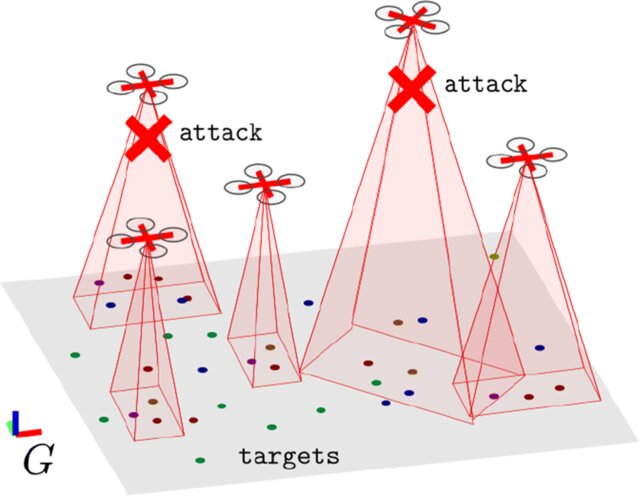
\includegraphics[width=0.7\textwidth]{figures/swarm2.jpeg}
    \end{subfigure}
    \begin{subfigure}[b]{0.49\textwidth}
        \centering
        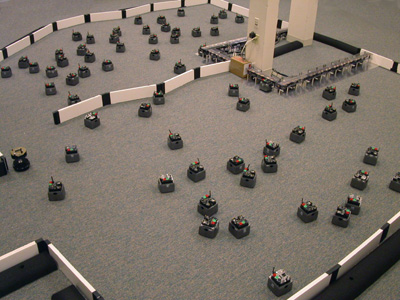
\includegraphics[width=0.6\textwidth]{figures/swarm3.jpeg}
    \end{subfigure}
    \begin{subfigure}[b]{0.49\textwidth}
        \centering
        
\includegraphics[width=0.7\textwidth]{figures/smartcity2.jpeg}
    \end{subfigure}
    \begin{subfigure}[b]{0.49\textwidth}
        \centering
        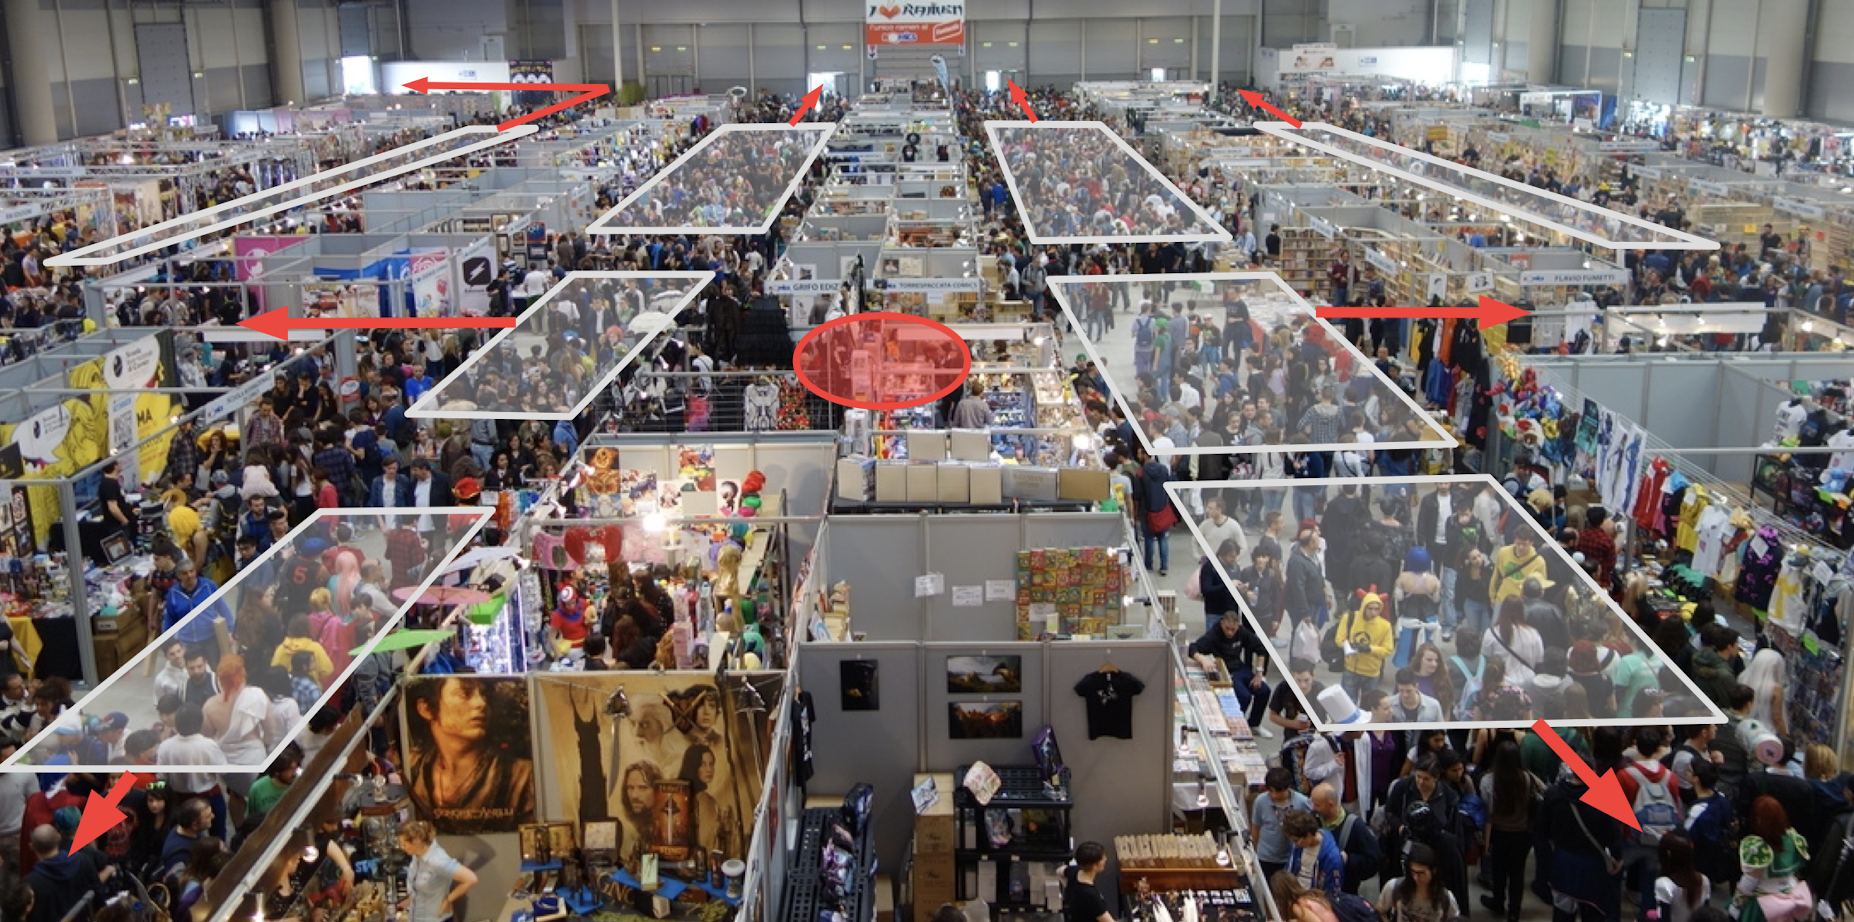
\includegraphics[width=0.7\textwidth]{figures/crowd.png}
    \end{subfigure}
    \caption{Some examples of Cyber-Physical Swarms.}%\vspace{-10pt}
    \label{fig:cpsw}
\end{figure*}


Swarms have been extensively studied due to a series of significant advantages, namely:
    i) \emph{cost}: the devices used are typically simpler than a single device that could solve the task individually, resulting in lower costs;
    ii) \emph{fault-tolerance}: simpler devices are less prone to failures, and there is no single point of failure;
    iii) \emph{scalability}: the system can be easily scaled by adding or removing devices;
    iv) \emph{robustness}: the system can handle the loss of some devices;
    v) \emph{flexibility}: the same system can solve different tasks.


%
\section{Aggregate Computing}

The advent of \emph{Collective Computing} and the proliferation of interconnected devices have given rise to novel 
    paradigms that aim to address the challenges posed by the distributed nature of computing
    systems. One such paradigm that has gained significant attention in recent years is 
    \emph{aggregate computing (AC)} \cite{AC}.

AC adopts a model where the perspective is at a \emph{global level}: 
    a group of devices is seen as a global entity (i.e., the \emph{aggregate system}) that works at asynchronous 
    \emph{rounds} and exchanges messages with neighbours. 
    A round is composed of three phases:
    i) \emph{context building}, each node collects information from the 
        neighborhood and sensors,
    ii) \emph{program execution}, each node executes the aggregate program on the local context, and
    iii) \emph{export sharing}, each node shares the export with the neighborhood.
    Each device is seen as an actor that has a set of responsibilities (\Cref{fig:device-actor}): first, it is equipped with 
    \emph{sensors} that allow it to detect certain characteristics of the environment and \emph{actuators} that allow 
    it to interact with the environment; furthermore, it must \emph{execute the collective program} specification 
    (asynchronously according to its clock) and keep track of the \emph{local state}. Lastly, it is equipped with 
    a \emph{communication mechanism} that enables it to exchange messages with other devices in its neighborhood.


\begin{figure}[t]
    \centering
    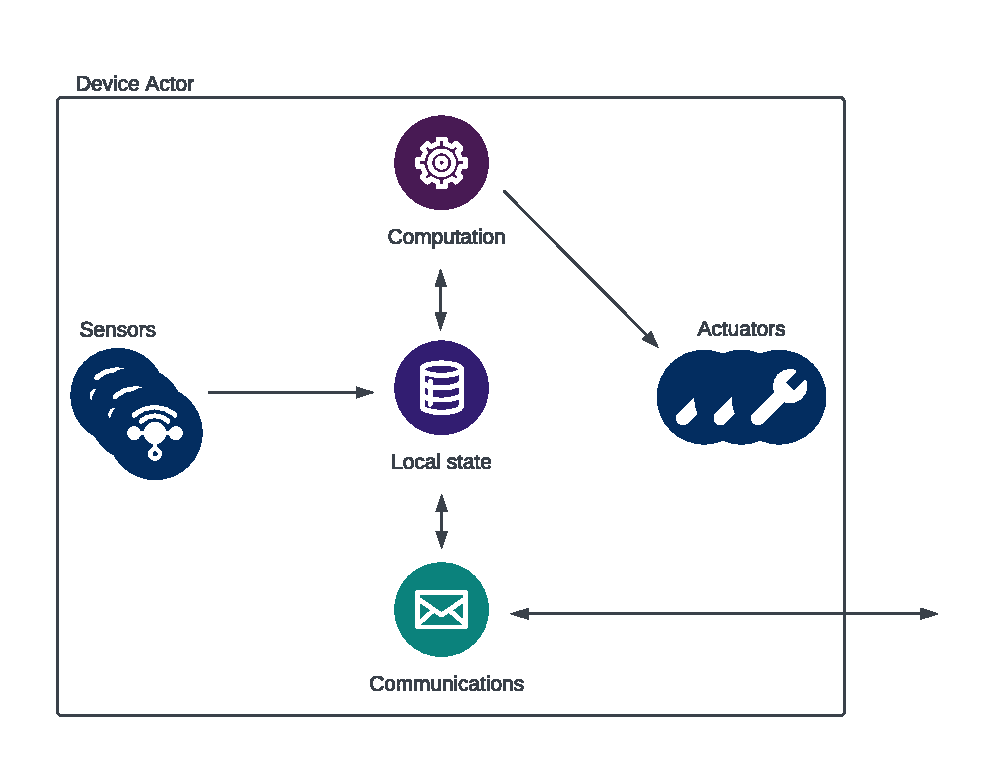
\includegraphics[width=0.7\textwidth]{figures/deviceactor.pdf}
    \caption{Device actor model in AC.}
    \label{fig:device-actor}
\end{figure}

Interactions within the aggregate system are seen as a flow of information propagating through the 
    collective of devices, rather than as local interactions of individual devices with their
    peers and the environment. This approach offers a number of advantages:
    i) the program can be defined in a composable and declarative manner, 
    ii) it promotes the reuse of behaviours, and 
    iii) the developer is relieved from concerns regarding low-level aspects (e.g., failures, distribution, communication and more), 
    as these are automatically handled by the middleware.

In aggregate computing, information is represented by a distributed data structure known as 
    \emph{computational field} \cite{VIROLI2019100486, 1316820},
    which is an abstraction of space-time values where each device is mapped to a computational value.
    The manipulation of these fields is derived from the \emph{Field Calculus} \cite{viroli2016higher}, a computational model in which collective 
    behaviours are expressed as algorithms that are the composition of computational fields.

In recent times, several implementations of aggregate computing have been developed, and one particularly interesting 
    implementation is \emph{ScaFi} \cite{CASADEI2022101248}. ScaFi is a Scala-based platform that offers the following features: 
    i) a domain specific language (DSL) for specifying aggregate computation, 
    ii) a simulation environment through the Alchemist simulator \cite{alchemist}, 
    iii) a middleware for executing and deploying aggregate programs, and 
    iv) reusable library functionalities that serve as building blocks for constructing new aggregate programs. 
    For example, the gradients abstraction that provides gradient functions \cite{viroli2018engineering, beal2008fast} used for the ongoing computation, 
    across spatio-temporal dimension, of the self-healing field (i.e., a field able to self-adjust in case of changes 
    in devices topology) that determines the minimum distances of individual nodes from a specified set of source 
    nodes \cite{CASADEI2022101248}.

An example of how ScaFi works is shown in \Cref{fig:channel} and \Cref{lst:channel}, the goal is create a channel given 
    a source, a destination and a width. To reach this goal is it possible to define the computation as a pure function 
    over fields that exploits and composes the following functions:
    i) \texttt{gradient}, which takes as input a field of Booleans and computes in output a field of Integers with the 
        mininum distance, for each point, from a given source represented by the values set to true in the input;
    ii) \texttt{distance}, which computes the distance between two sources, and
    iii) \texttt{dilate}, which takes as input a field of Booleans and stretches the source by a given width.

\begin{figure}[h!]
    \centering
    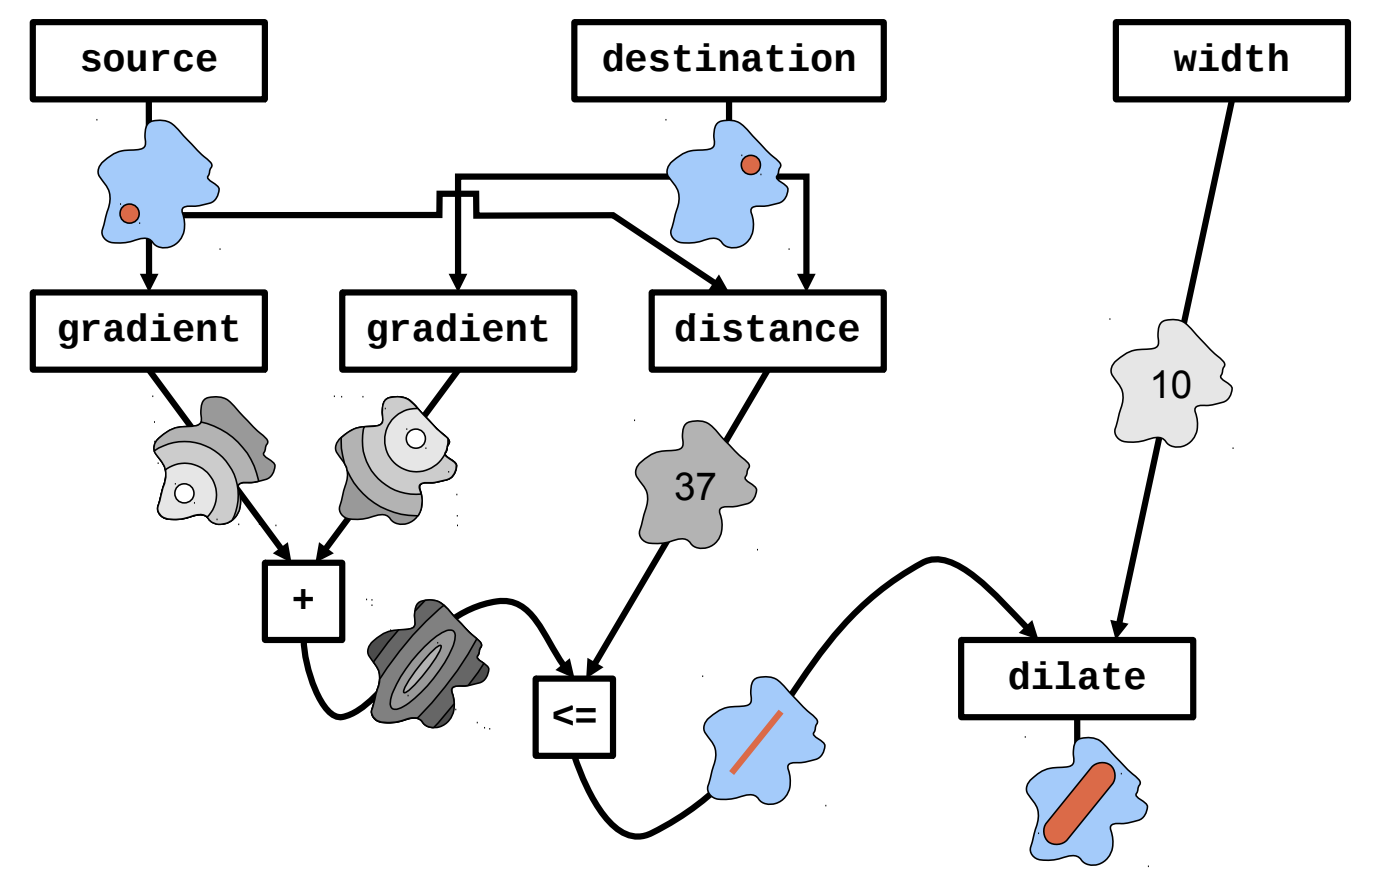
\includegraphics[width=0.7\textwidth]{figures/channel.png}
    \caption{A ScaFi AC program example. This algorithm representation is obtained from the code in \Cref{lst:channel}}.
    \label{fig:channel}
\end{figure}

\begin{lstlisting}[caption={A ScaFi AC program example. The algorithm implements a channel between a source and a destination.}, label={lst:channel}]
def channel(
    source: Boolean, 
    destination: Boolean, 
    width: Double
): Double {
    dilate(gradient(source) + gradient(destination) 
        <= distance(source, destination), width)
}
\end{lstlisting}

%
\section{Reinforcement Learning}
%

``\emph{Reinforcement Learning (RL)} is the science of decision making. It is about learning the optimal behavior 
    in a environment to obtain maximum reward" 
    \footnote{\url{https://www.synopsys.com/ai/what-is-reinforcement-learning.html}}.
    RL is a general framework, other than supervised and unsupervised learning, in which an \emph{agent} learns 
    to behave within an \emph{environment} by performing some \emph{actions} and seeing the result they produce.
    It is inspired by how humans and animals learn through the system of rewards and punishments: for each good action
    the environment provides to the agent a positive reward, instead, for each bad action the agent gets a negative 
    reward (also called penalty).

Formally, a RL problem can be formulated as following \cite{RLSurvey}:
    \begin{itemize}
        \item Discrete time steps $t=0, 1, 2, ...$;
        \item A discrete set of environment states $\mathcal{S}$;
        \item A discrete set of agent actions $\mathcal{A}$;
        \item A reward signal;
        \item A probabilistic policy $\pi$, that is a mapping function from states to actions.
    \end{itemize}
    The goal of the agent is to learn the optimal policy $\pi^*$ in order to maximize 
        some long-run measure of reinforcement (e.g., the Infinite Horizon Discounted Model \cite{RLSurvey}).
        First, at time $t$, the agent observes the state of the environment $s_t \in \mathcal{S}$
        and chooses an action $a_t \in \mathcal{A}$ using the actual policy $\pi_t$. 
        Thereafter, the environment: takes in the action $a_t$, emits the new state $s_{t+1} \in \mathcal{S}$ 
        and returns the scalar reward $r_{t+1}$ (\Cref{fig:rl_schema}).
        Finally, the agent, based on the reward obtained updates its knwoledge.
    This formulation stems from \emph{Markov Decision Processes}, which is a mathematical framework for \emph{sequential decision making}. A very important property that these systems must adhere to is the \emph{Markov property}, which states ``\emph{the future is independent of the past given the present.}" In other words, it implies that the state transition function does not require the entire past trajectory but only the last state, namely: 
    $$p(s_{t+1} | s_t, a_t, ..., s_0, a_0) = p(s_{t+1} | s_t, a_t)$$
    It is important to note that the concept of state can always be extended to satisfy this property.


\begin{figure}[t]
    \centering
    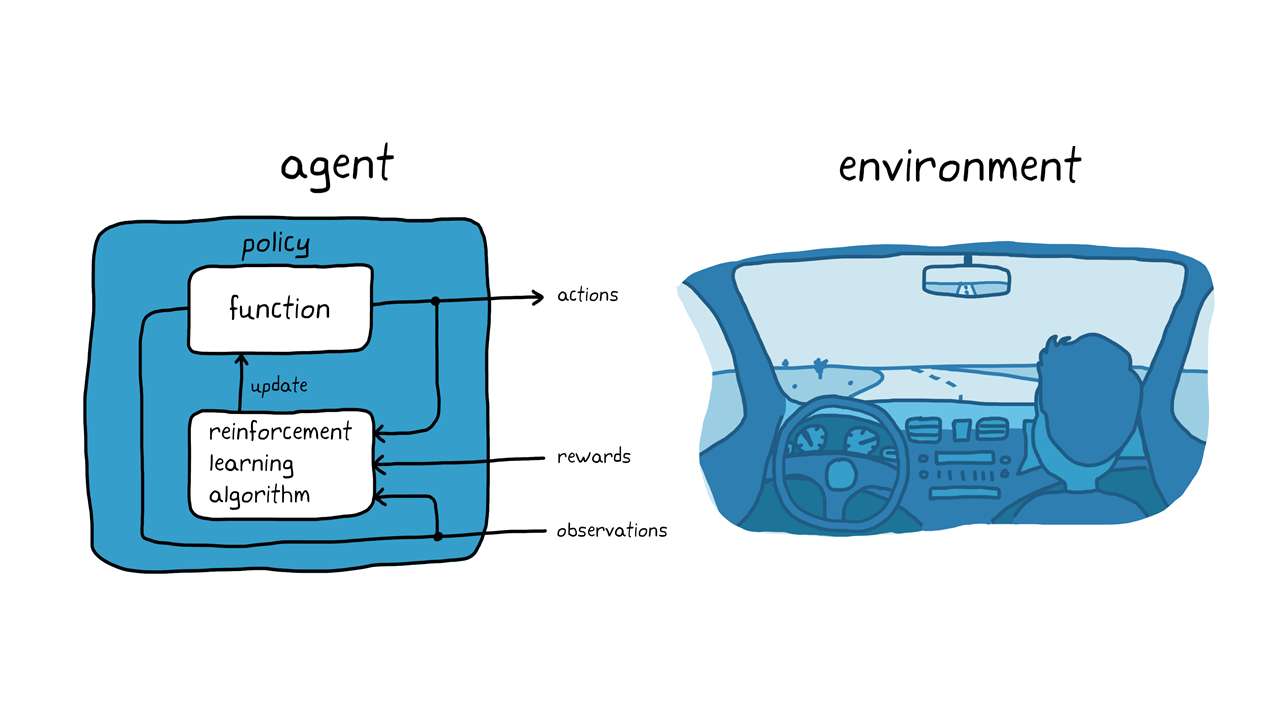
\includegraphics[width=0.7\textwidth]{figures/rl.png}
    \caption{Agent-environment interactions.}
    \fonte{\url{https://it.mathworks.com/discovery/reinforcement-learning.html}}
    \label{fig:rl_schema}
\end{figure}

In order to find the optimal policy $\pi^*$, the agent tries to maximize the expected cumulative reward.
    Since the environment is stochastic (i.e., the same action performed in the same state could lead to different 
    results over time) the more you look into the future the more the outcome could diverge.
    For this reason, it is common to use a model that takes less account of rewards that are far away in time 
    than those that are close in time:
    $$R_t = \sum_{i=t}^{\infty} \gamma^{i-t} \cdot R_{\pi(s_i)}(s_i, s_{i+1}) $$
    This model is called \emph{Infinite Horizon Discounted Model}, the key aspect is the hyper-parameter $\gamma$.
    It is a scalar weight in the range $[0;1]$, in this way, the further away the reward is in time, the smaller its weight.

\paragraph{Exploration-exploitation dilemma}

The \emph{exploration-exploitation dilemma} is a problem that comes from the definition of the RL process.
    In order to increase its knowledge and build an optimal policy, the agent needs to \emph{explore} the environment 
    in the hope of finding better actions. After some exploration, the agent might have found a set of 
    apparently rewarding actions, but, how can the agent be sure that the found actions are actually the best? 
    When should the agent continue to explore or else, when should it just \emph{exploit} its existing knwoledge?

Several exploration strategies have been proposed in the literature to solve this problem, the simplest is the
    \emph{$\epsilon$-greedy} strategy. The agent \emph{randomly explore} the environment with probability $\epsilon$
    while \emph{exploit} the current optimal action with probability $1-\epsilon$.

    $$
    \pi(s)=
    \begin{cases}
        \pi^*(s) & \text{with probability $1-\epsilon$} \\
        \text{\emph{random action}} & \text{with probability $\epsilon$}\\
    \end{cases} 
    $$ 

    Usually, at the beginning of the learning process $\epsilon$ starts near to $1$ (i.e., more exploration) and then decreases
    to $0$ as the agent learns more and more about the environment. 

\paragraph{Main approaches}

In Reinforcement Learning, there are two main families of approaches that can be used to categorize the 
    algorithms employed by an agent in finding the optimal policy. These are: 
    i) \emph{policy-based} methods, and 
    ii) \emph{value-based} methods.
    Policy-based algorithms aim to directly learn a function that maps each state to the best action to take 
    (or a probability distribution over a set of possible actions). On the other hand, value-based methods 
    seek to learn a function that maps each possible state to an expected value of being in that state. 
    This way, the agent can learn which states is more valuable and will take action that leads to it. 
    This comparison is well illustrated in \Cref{fig:rl-methods}.

An example of policy-based method is \emph{Proximal Policy Optimization (PPO)} \cite{ppo}, while an example of 
    value based-method is \emph{Q-Learning} \cite{QL}

\begin{figure*}[t]
    \begin{subfigure}[b]{0.49\textwidth}
        \centering
        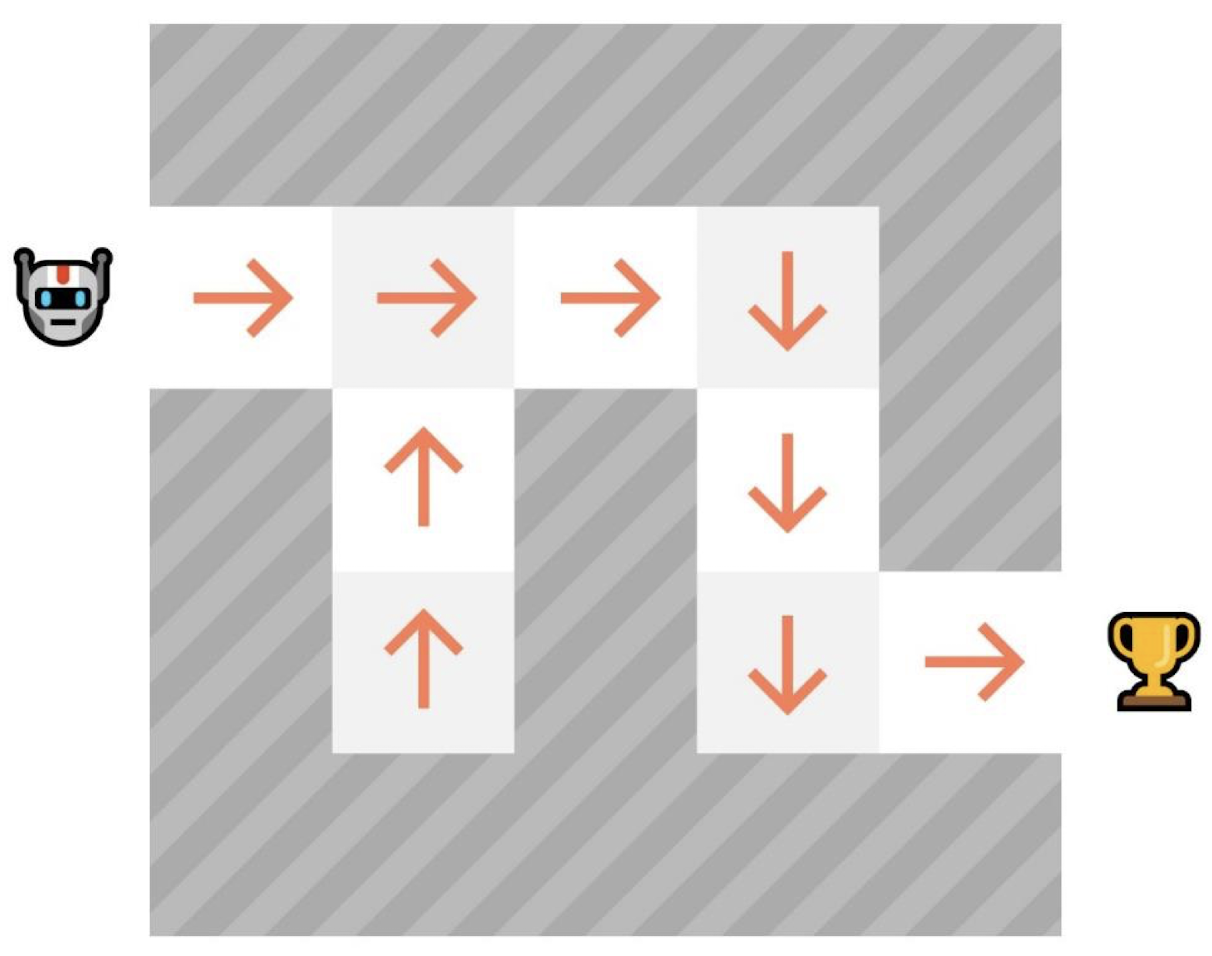
\includegraphics[width=0.7\textwidth]{figures/policy-based-rl.png}
        \caption{Policy based RL}
        \label{fig:policy-based-rl}
    \end{subfigure}
    \begin{subfigure}[b]{0.49\textwidth}
        \centering
        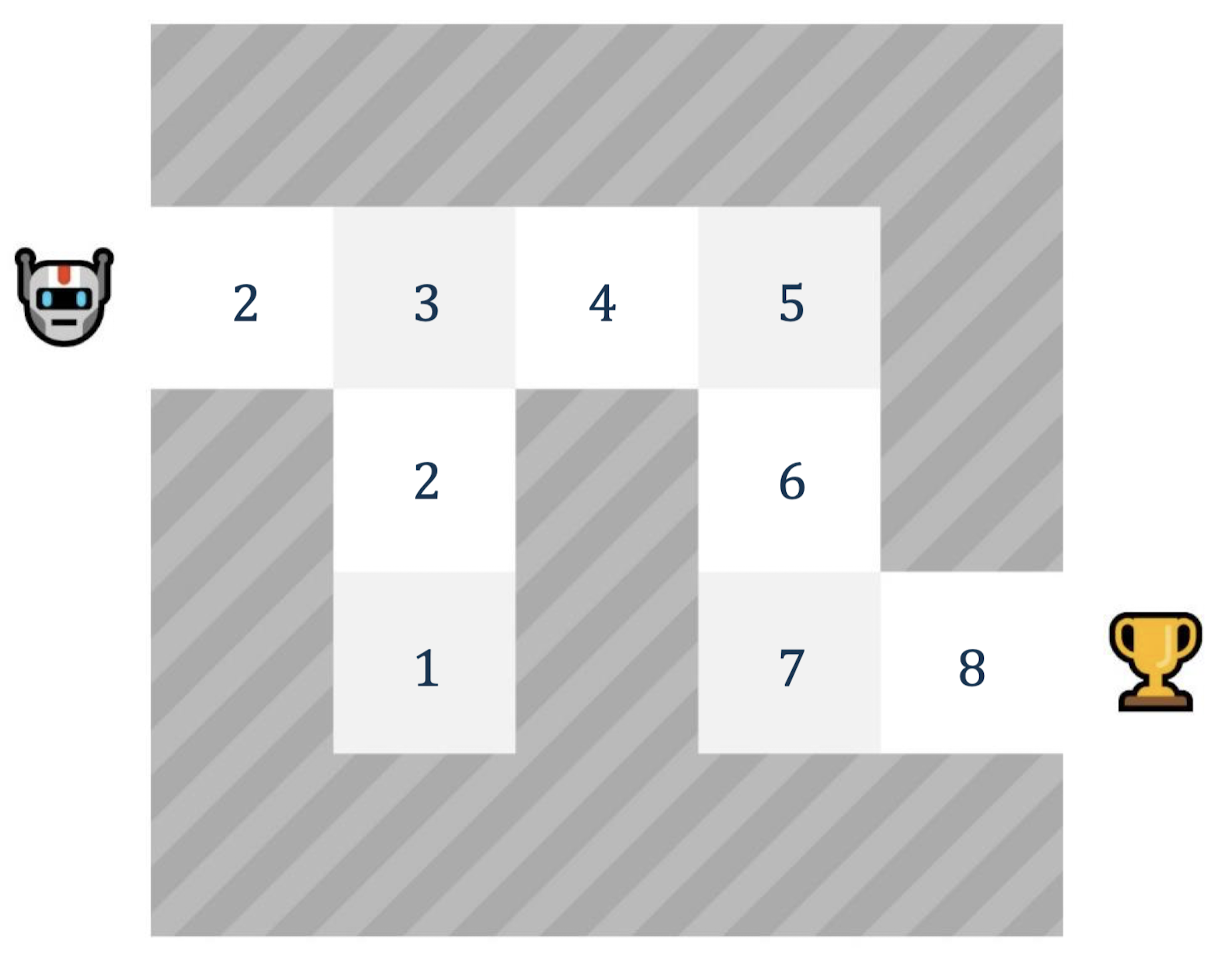
\includegraphics[width=0.7\textwidth]{figures/value-based-rl.png}
        \caption{Value based RL}
        \label{fig:value-based-rl}
    \end{subfigure}
\caption{Policy and value based algorithms visual comparison.}%\vspace{-10pt}
\fonte{\url{https://www.lamsalashish.com.np/blog/reinforcement-learning}}
\label{fig:rl-methods}
\end{figure*}

\paragraph{Q-Learning}

\emph{Q-Learning} is one of the most famous Reinforcement Learning algorithm from the value-based methods family. 
    One of the key aspects of this algorithm is the \emph{Q-Table}, denoted as $Q(s,a)$. This table represents, 
    for each possible state-action pair, the \emph{expected cumulative reward} that the agent will obtain by
    taking action $a$ in state $s$ and subsequently following optimal actions. 
    Thus, the Q-table at time step $t$, given a state $s_t$, an action $a_t$, and a policy $\pi_t$, is represented by:
    $$ Q(s_t, a_t) = max_{\pi(s_t) = a_t} R_{t+1}$$
    Starting from the Q-Table, it is possible to define the \emph{optimal policy} as follows:
    $$ \pi^{*}(s) = argmax_a Q^{*}(s,a) $$

Another key aspect is how we can estimate the reward at the end of the process if we only know the current state 
    and action, without knowing the subsequent trajectory. To achieve this, the \emph{Bellman equation} can be used. 
    This equation defines, for a given transition $<s_t, a_t, s_{t+1}, r_{t+1}>$, the value $Q(s,a)$ recursively 
    as the sum of the immediate reward and the maximum expected cumulative reward from the subsequent state:
    $$ Q(s_t,a_t) =  r_{t+1} + \gamma \cdot max_a Q(s_{t+1}, a)$$

The main idea of Q-Learning is to \emph{iteratively approximate} the Q-values, using the Bellman equation, as follows:
\[
Q(s_t,a_t) = 
    \underbrace{
        (1-\alpha) 
    }_\text{Learning Rate}   
    \cdot 
    \underbrace{
        Q(s_t,a_t) 
    }_\text{Old Value}
    + 
    \underbrace{
        \alpha
    }_\text{Learning Rate}
    \cdot 
    \overbrace{
        (
        \underbrace{
            r_{t+1}
        }_\text{Reward}
        + 
        \underbrace{
            \gamma
        }_\text{Discount Factor}
        \cdot 
        \underbrace{
        max_a Q(s_{t+1}, a)
        }_\text{Maximum Future Reward}
        )
    }^\text{Learned Value}
\]
    Where $\alpha$ is the learning rate hyper-parameter that controls how much of the current Q-value and newly proposed
    Q-value is considered.
    At the beginning of the learning process, these Q-values will be practically random estimates and may be completely wrong. 
    However, it has been demonstrated that as iterations progress, these Q-values will 
    converge and represent the true Q-values.

\paragraph{Deep Reinforcement Learning}

Classical algorithms of reinforcement learning, when applied in \emph{real-world contexts}, suffer from the problem of \emph{state space explosion}.
    This arises from an exceedingly large number of possible states, making the resolution of a given task \emph{computationally intractable}. 
    For instance, in the game of chess, there can be around $100^{100k}$ possible games, a number much larger than 
    the count of sand grains on Earth ($\approx 10^{23}$) and the number of atoms in the observable universe 
    ($\approx 10^{81}$). 
    For this reason, \emph{deep reinforcement learning} has been introduced, which involves utilizing deep neural networks
    as approximators for the policy and/or the value function.

One of the most well-known Deep RL algorithms is DQN \cite{dqn}. This was developed by DeepMind in 2013 and was initially
    used to train an agent capable of playing Atari video games. One of the advantages of using neural networks as 
    approximators for the function to be learned is the ability to avoid hand-engineering the state space and instead 
    allow the network to learn the best features directly. For example, in the case of Atari games, this is achieved 
    by using convolutional layers and feeding the network with screen raw pixels.
    
DQN, specifically, is the deep version of the Q-Learning algorithm, thus producing a Q-Value output for each 
    possible action (\Cref{fig:qlvsdqn}). This makes the training of the utilized neural network a regression task 
    in which a squared error loss can be employed as the loss function:
    $$ L = (y_t - \hat{y_t})^2 $$
    Where $y_t$ represents the actual value and $\hat{y_t}$ is the predicted value at time t. Since RL is an 
    unsupervised learning, and therefore labels are not available, the value $y_t$ is estimated using the 
    Bellman equation, transforming the loss function for a transition $<s_t, a_t, s_{t+1}, r_{t+1}>$ into:
    $$ L = ( r_{t+1} + \gamma \cdot max_a Q(s_{t+1}, a) - Q(s_t, a_t))^2 $$

\begin{figure*}[t]
    \begin{subfigure}[b]{0.49\textwidth}
        \centering
        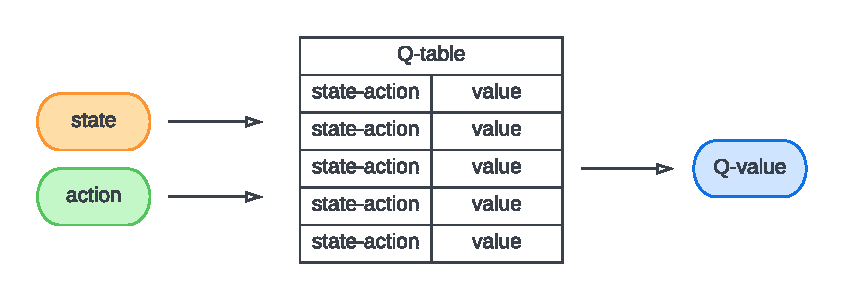
\includegraphics[width=\textwidth]{figures/q-learning.pdf}
        \caption{Q-Learning}
        \label{fig:ql}
    \end{subfigure}
    \begin{subfigure}[b]{0.49\textwidth}
        \centering
        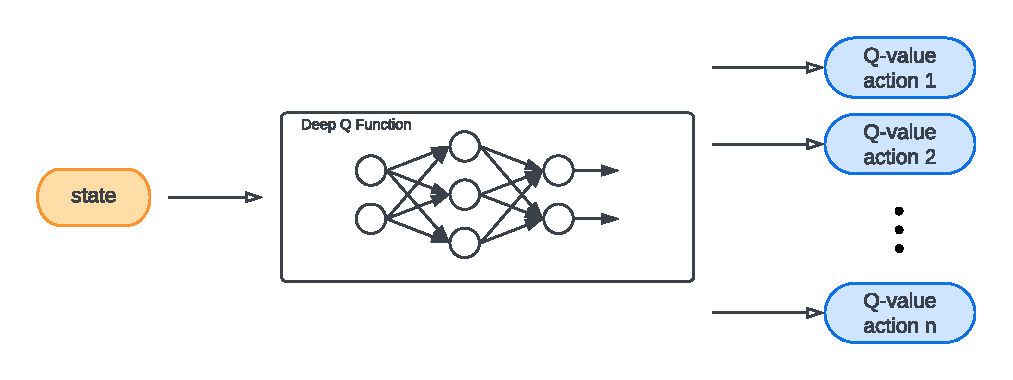
\includegraphics[width=\textwidth]{figures/deepQL.pdf}
        \caption{Deep Q-Learning}
        \label{fig:dqn}
    \end{subfigure}
\caption{Q-Learning and Deep Q-Learning visual comparison}\vspace{-10pt}
\label{fig:qlvsdqn}
\end{figure*}

When attempting to use neural networks to approximate the Q-function, several problems arise. 
    The first one is due to the high correlation that exists between two consecutive transitions within the same 
    episode. This correlation leads to a significant decrease in variance, causing the network to tend to forget 
    previous transitions as it overwrites them with newer ones. For instance, let's consider an agent's task to 
    learn to play a level-based video game; this issue implies that while the agent tries to learn how to navigate 
    the second level, it might forget how to behave in the first level. The most common solution is to employ an 
    \emph{experience replay} (i.e., a buffer), where all transitions $<s_t, a_t, s_{t+1}, r_{t+1}>$ are stored. 
    When updating weights, a random mini-batch is sampled from this buffer, breaking the correlation between consecutive
    transitions. Furthermore, since a transition can be used in multiple weight updates, this approach also 
    improves data efficiency.

A second issue that can be observed is referred to as the \emph{moving target problem}. This stems from the fact that,
    when updating the network's weights, both the predicted values and the target values are estimated using the 
    same neural network. This leads to a strong correlation between the target values and the network's weights, 
    introducing significant oscillations during training. To address this problem, two distinct neural networks 
    with identical architecture are employed: 
    i) \emph{the action network $Q$}, used to determine the agent's actions, which is updated every $u$ steps; 
    ii) \emph{the target network $\hat{Q}$}, used to calculate the target values, updated every $c$ steps. 
    Typically, $c >> u$, and the \emph{target network's} weight update involves replacing the existing weights with 
    those from the \emph{action network}.
    Since the target values are generated using an older set of weights, a delay is introduced between the 
    moment the $Q$ network is updated and the moment it starts to affects the target values.
    This delay reduces the likelihood of divergence and oscillations. The loss function becomes:
    $$ L = ( r_{t+1} + \gamma \cdot max_a \hat{Q}(s_{t+1}, a) - Q(s_t, a_t))^2 $$

\section{Multi-Agent Reinforcement Learning}
\emph{Multi-Agent Reinforcement Learning} is an extension of RL where multiple agents interact one another and 
    with the environment. 
    Usually, MARL is modelled as a \emph{Markov Game} (or Stochastic Game $\mathcal{S}$)~\cite{LITTMAN1994157} in
    which we have:
    \begin{itemize}
        \item A tuple $\mathcal{S} = <N, S, \{A^i\}, P, \{R^i\}>$ with $i \in 1 \dots N$
        \item The number of agents $N > 1$
        \item The action space of the i-th agent $A^i$. The global action space is defined as $\mathbb{A} = A^1 \times A^2 \times \dots \times A^N$
        \item A function describing the transition dynamics $P: S \times \mathbb{A} \rightarrow \mathcal{P}(S)$
        \item The reward function $R^i: S \times \mathbb{A} \times S \rightarrow \mathbb{R}$ for each agent $i$ 
    \end{itemize}

\paragraph{Categorization}

Based on the reward function used by the agents, MARL can be divided into two categories: 
    i) \emph{cooperative}, where all the agents trying to maximize the same reward function (e.g., a group of robots
    trying to clean a room); 
    ii) \emph{competitive}, where, potentially, each agent has its own reward function that is conflictual with the other (e.g., a rock-paper-scissor game). 
    Cooperative MARL, with respect to the policy, can be further divided into two additional categories, namely: 
    i) \emph{homogeneous}, where all the agents have the same capabilities, i.e., they use the same policy 
    ii) \emph{heterogeneous}, where each agent may have its own policy, in this case, each agent tries to maximize the local policy following the global shared goal.

In this thesis, we focus on a subset of MARL, namely: \emph{Many Agent Reinforcement Learning}~\cite{yang2021many}. The only
    difference between the two approaches is in the number of agents involved. 
    Typically, in Many Agent Reinforcement Learning the number of agents may range from a hundred to one or two
    thousands whereas, in Multi Agent Reinforcement Learning, there are only a few tens~\cite{smac,marl-curricula}.
    Moreover, we focus on cooperative homogeneous and heterogeneous learning.


\paragraph{Training and execution model}
   
Another point to pay attention to is the system by which the training and execution of the various agents are carried out. This can be primarily categorized into three types (\Cref{fig:exmod}):
    i) \emph{Centralized Training Centralized Execution (CTCE)}, in this type of system, there is a higher-level agent called \emph{Learner}, with a global perspective, whose task is to perform training and compute actions to be undertaken. The remaining agents, therefore, transmit their local environmental perceptions (i.e., the local state) to the learner agent, which is responsible for merging these perceptions to reconstruct the global state. Once reconstructed, it selects the action to take in accordance with the current policy and evaluates the reward function for policy updates;
    ii) \emph{Centralized Training Decentralized Execution (CTDE)}, in this type of system, a learner agent with a global perspective executes the training algorithm. Once the policy is updated, it is sent to each agent, which can interact with the environment and take actions in accordance with it;
    iii) \emph{Decentralized Training Decentralized Execution (DTDE)}, in this type of system, each agent has its own local policy and can only observe a portion of the environment. Each agent, therefore, takes actions based on its perception of the environment and updates its own local reward function accordingly.

\begin{figure*}[t]
    \begin{subfigure}[b]{0.32\textwidth}
        \centering
        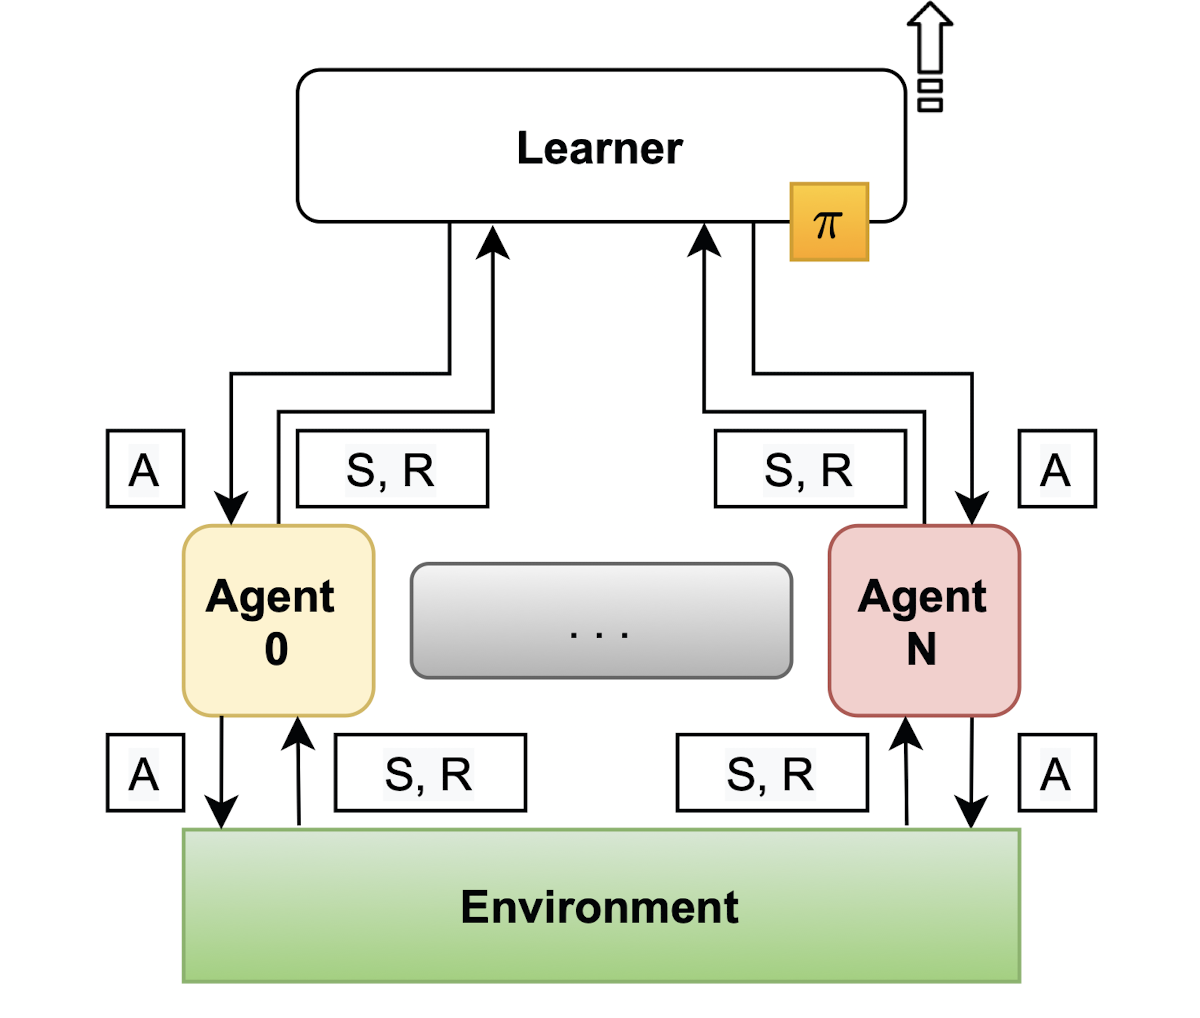
\includegraphics[width=\textwidth]{figures/CTCE.png}
        \caption{CTCE}
        \label{fig:ctce}
    \end{subfigure}
    \begin{subfigure}[b]{0.32\textwidth}
        \centering
        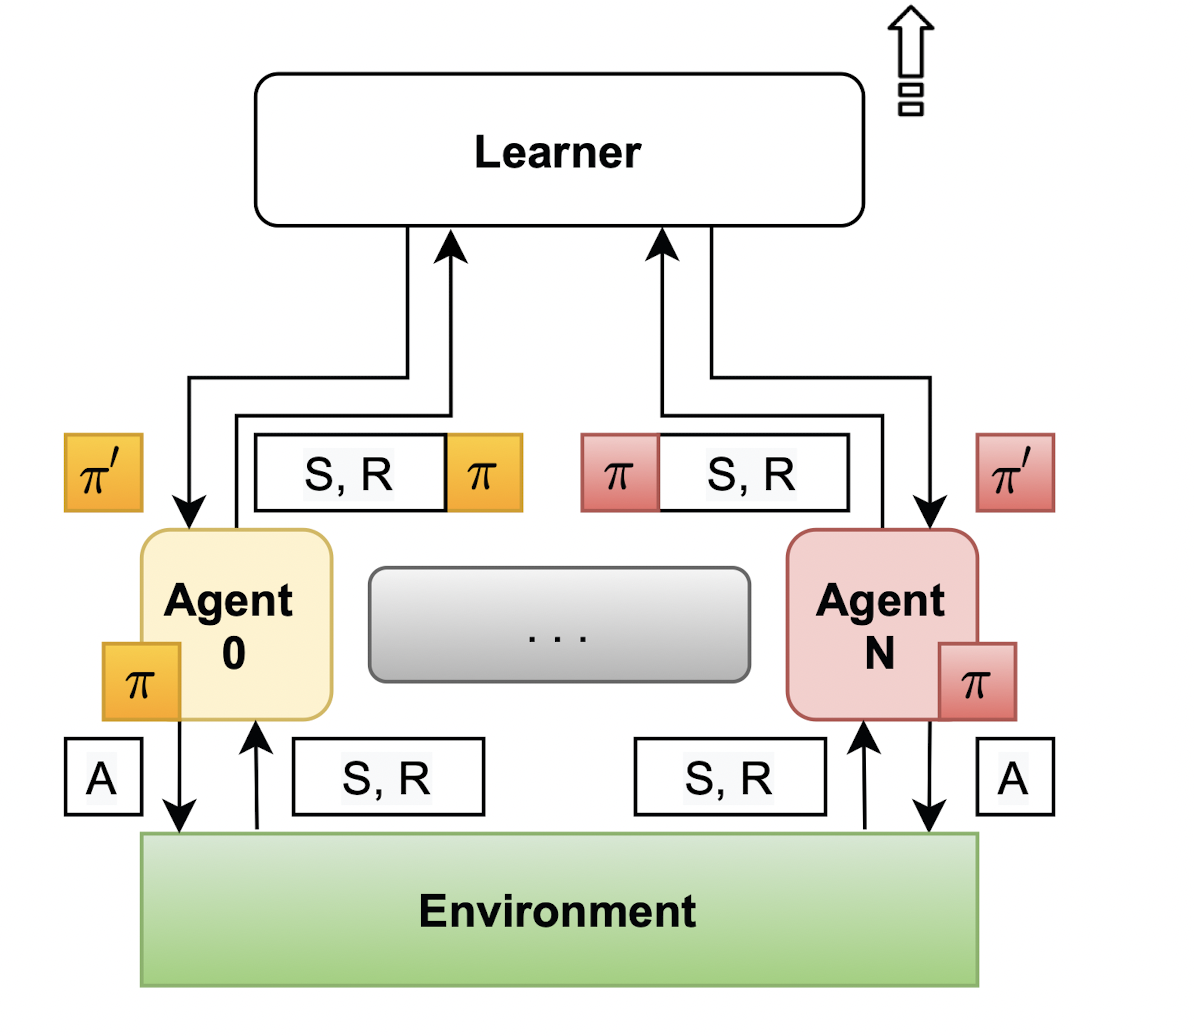
\includegraphics[width=\textwidth]{figures/CTDE.png}
        \caption{CTDE}
        \label{fig:ctde}
    \end{subfigure}
    \begin{subfigure}[b]{0.32\textwidth}
        \centering
        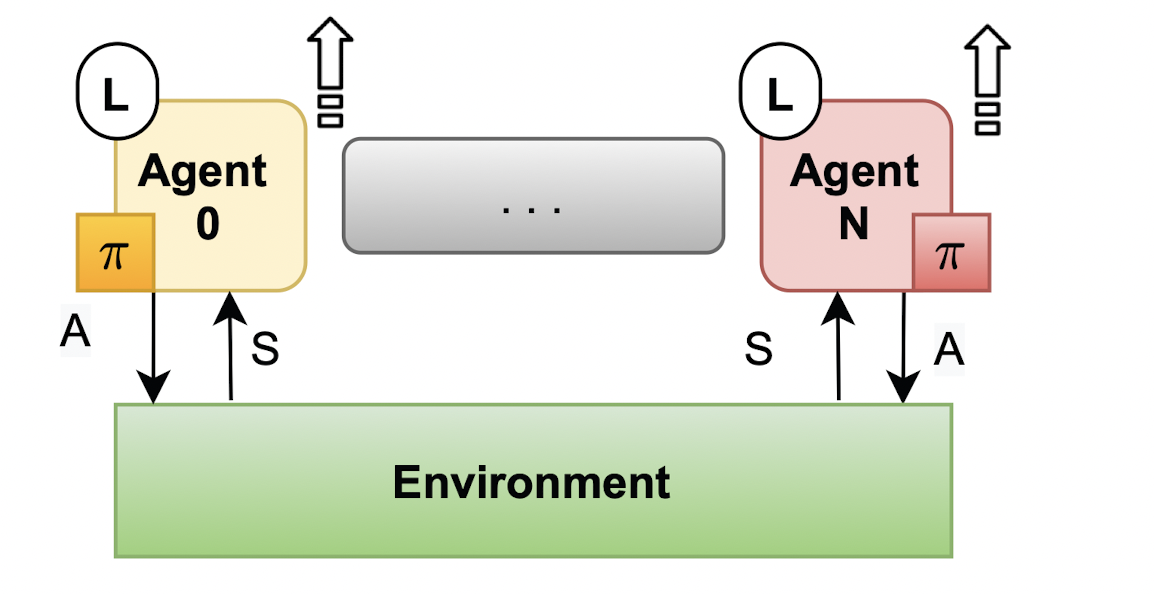
\includegraphics[width=\textwidth]{figures/DTDE.png}
        \caption{DTDE}
        \label{fig:dtde}
    \end{subfigure}
    \caption{MARL execution model comparison.}\vspace{-10pt}
    \label{fig:exmod}
\end{figure*}

\paragraph{Challenges}

MARL is a highly promising field that has been garnering increasing attention in recent years. Nevertheless, there are still several challenges that complicate its application in complex contexts. Some of these challenges include:
\begin{enumerate}
   

    \item  \emph{Partially Observable Environments}: in environments of significant complexity, agents cannot have a complete representation of the surrounding environment nor access the state of other present agents.
   
    \item \emph{Non-Stationarity}: this issue arises due to multiple agents simultaneously learning and changing the environment. From the perspective of an individual agent, the environment becomes non-stationary.
   
    \item  \emph{Agent Communication}: communication among agents is a crucial feature in the literature. The problem not only addresses what an agent should communicate but also with whom and when.
   
    \item  \emph{Coordination}: coordination is essential in cooperative systems, as agents must reach a consensus on the actions to take. Failure to coordinate during learning can lead to suboptimal policies. Coordination can be achieved through communication or implicitly, with each agent constructing its own model of other agents' behavior to infer their next actions.
   
    \item  \emph{Credit Assignment Problem}: this refers to associating a reward with an action taken by a specific agent. This association is crucial for learning to understand the effectiveness of an action and maximizing the reward function over time.
   
    \item  \emph{Scalability}: the scalability of these systems is influenced by the challenges outlined in this section. Training a single agent is inherently challenging; as the number of agents in the system increases, the complexity grows exponentially. Additionally, scalability is determined by an agent's robustness in the face of changes in the behavior of other agents. Literature presents exploration techniques to enhance scalability, such as knowledge reuse, regularization, adversarial training, and others.
\end{enumerate}

\section{Simulation}

In science and engineering, the use of \emph{simulators} plays a key role. These simulators enable the experimentation 
    with complex and expensive systems (such as cyber-physical swarms), offering a virtual 
    environment in which to conduct tests, analyses, and in-depth studies rapidly, under controlled and 
    repeatable conditions.
    In this project, the \emph{Alchemist} \cite{alchemist} simulator has been taken as a reference.

Alchemist is a \emph{meta-simulator} designed for simulating \emph{complex distributed systems} in a rich variety of scenarios 
    like swarm robotics \cite{Casadei2021}, large-scale sensor networks \cite{Aguzzi_2022},
    crowd simulation \cite{Beal2015}, path planning, and even morphogenesis of multi-cellular systems.

This simulator is ``meta" \emph{by design}, this stems from the fact that it is based on general abstractions that
    can be mapped to specific use cases (i.e., \emph{incarnations}). The meta-model is inspired by biochemistry
    and consists of a set of \emph{nodes} that exist in an \emph{environment} and are linked together by 
    \emph{relationship} rules.
    Each node contains a sequence of \emph{molecules} and \emph{reactions}. 
    A \emph{molecule} represents a variable, which acts as a container for data. 
    \emph{Reactions} instead are events that occur based on a set of \emph{conditions}, and are fired according 
    to a time distribution, producing an effect that is described as an action. 
    This abstraction allows the simulator to be flexible and adaptable to a variety of use cases and node
    numbers (it could support thousands of nodes), while maintaining a consistent underlying structure

Alchemist features four incarnations: biochemistry, sapere, protelis, and ScaFi, 
    each with a different way of modeling molecules and actions.
    In this project, the \emph{ScaFi} incarnation has been taken as a reference.
    It supports the ScaFi Scala DSL and has been used in distributed peer-to-peer chats and 
    situated problem-solving

Alchemist offers an straightforward method for defining simulations. The process
    requires a YAML file that includes essential parameters, such as the incarnation
    type, neighbor connection model, and node deployment. In Figure 2, we have
    provided an example YAML file that creates a simulation using the ScaFi incarnation (first row). It also defines the neighborhood relationship based on fixed
    distances (0.5 in this case), placing nodes in a fixed grid of size 10x10 starting
    at -(5,5) and ending at (5,5), with a node-to-node distance of 0.25. Finally, it
    loads the ScaFi program called ``program", which is evaluated at each node with
    a frequency of 1.

\begin{figure*}
    \centering
    \begin{subfigure}[b]{0.49\textwidth}
        \centering
        \begin{lstlisting}[language=yaml]
    incarnation: scafi
    network-model:
        type: ConnectWithinDistance
        parameters: [0.5]
    deployments:
        type: Grid
        parameters: [-5,-5,5,5,0.25,0.25]
        /*dynamics of the simulation*/
        programs: 
            - program:
            - time-distribution: 1
                type: Event
                actions: 
                - type: RunScafiProgram
                    parameters: [program]
            - program: send
    \end{lstlisting}
    \end{subfigure}
    \hfill
    \begin{subfigure}[b]{0.49\textwidth}
        \centering
        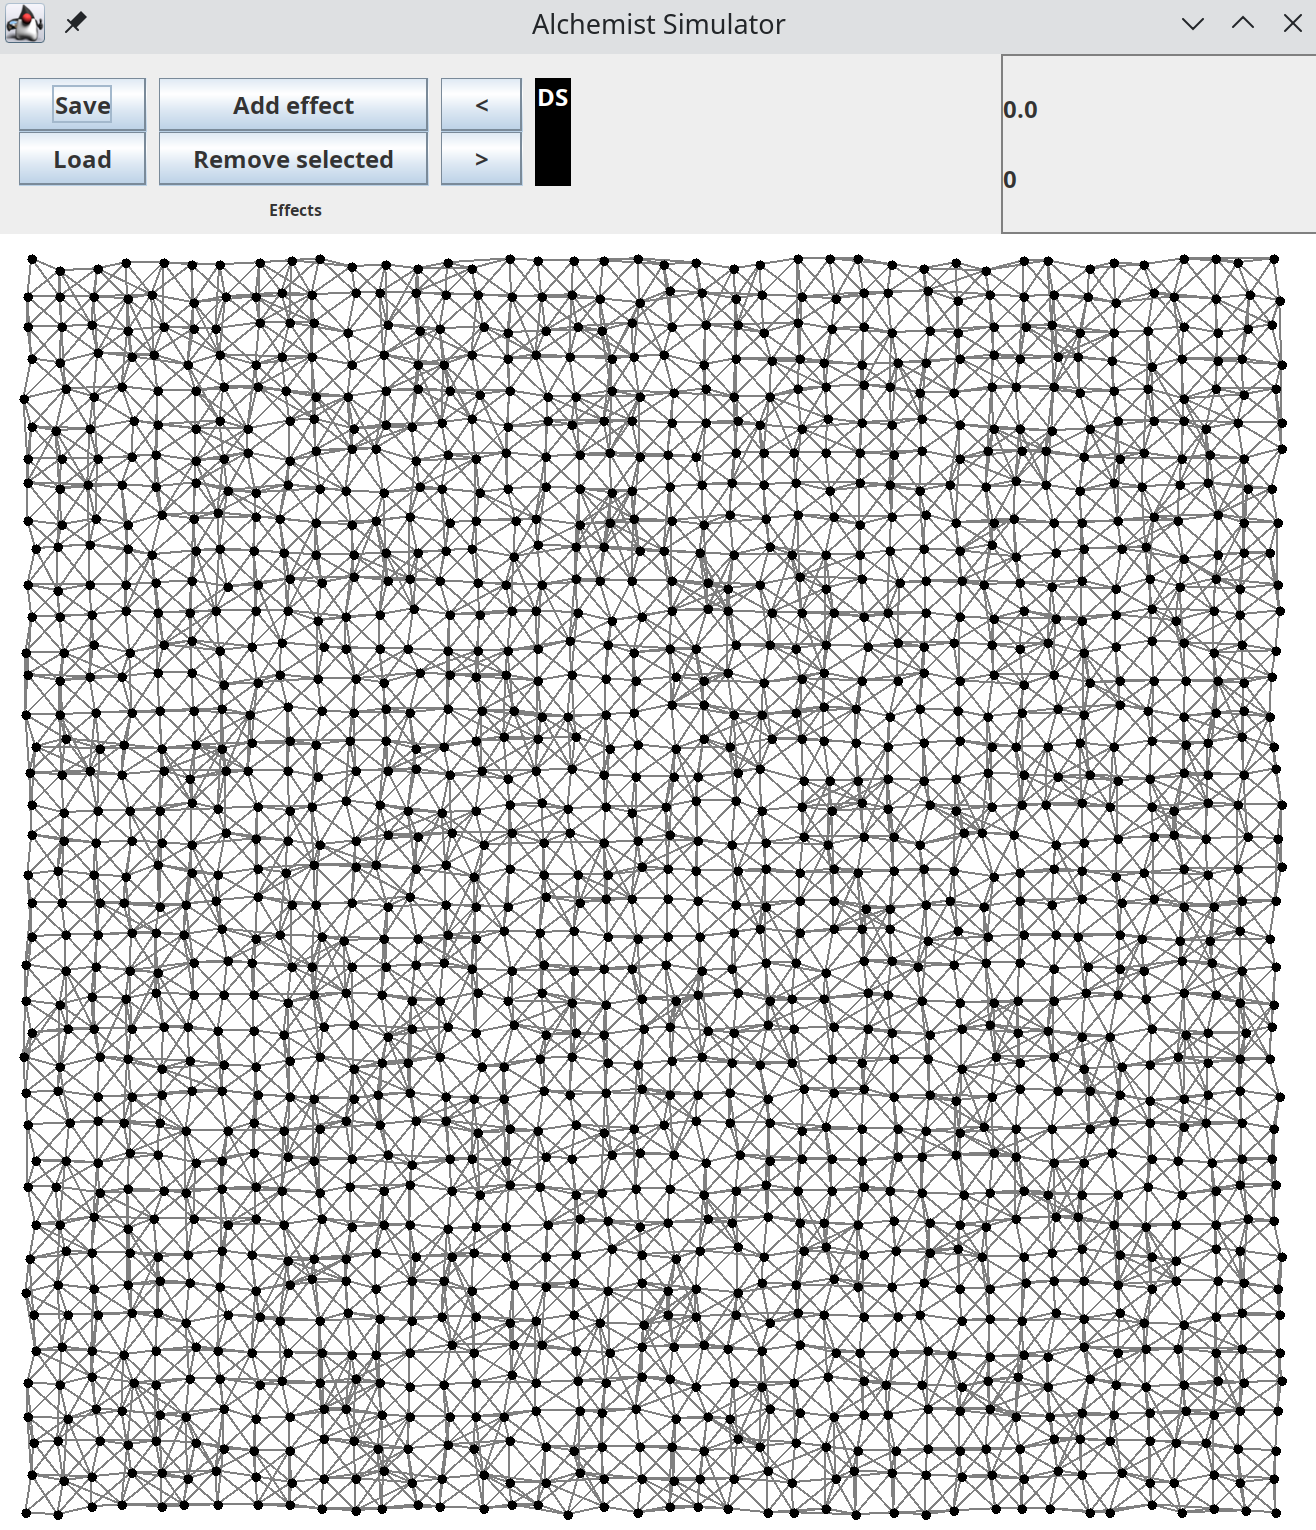
\includegraphics[width=\textwidth]{figures/alchemist.png}
    \end{subfigure}
    \caption{An Alchemist simulation example.}
    \label{fig:alchemist}
    \end{figure*}
%----------------------------------------------------------------------------------------
\chapter{Requirements} 
\label{chap:requirements}
%----------------------------------------------------------------------------------------
This chapter first introduces the domain model of the \emph{hybrid AC-MARL} approach to engineer CPSWs, 
    and then presents the framework requirements. Finally, some scenarios
    are explained to provide a reference context.

\section{Domain model}
The proposed \emph{hybrid} approach between \emph{AC} and \emph{MARL} aims to combine the strengths of the two 
    approaches to engineer CPSWs.
    The idea is to leverage AC to define \emph{structural} rules of the swarm (e.g., leader election \cite{pianini2022self}) 
    while using MARL to define \emph{behavioral} rules (e.g., the choice of an action by an agent).
    Harnessing machine learning allows for the definition of more complex and adaptive behaviors, 
    which would be challenging to achieve through programmatic methods.

To accurately define the domain, a \emph{Domain-Driven Design} \cite{evans2004domain} approach was used. 
    First, the \emph{ubiquitous language}, as presented in \Cref{tab:ul}, was defined. 
    This associates a precise definition with each term of the domain, thereby 
    eliminating potential \emph{ambiguities}, which are common given the breadth of the MARL domain.

\begin{table}
    \centering
    \begin{tabularx}{\textwidth}{lX}
        \hline
        \textbf{\emph{Concept}} & \textbf{\emph{Definition}} \\
        \hline
        Environment & The context in which the \emph{agents} are immersed and operate,
                        it is a representation of the task to be solved.
                        It is capable of interacting with the agents, providing information
                        about its current \emph{state}, receiving the \emph{actions} that one or more agents
                        wish to execute, and returning the corresponding \emph{reward}. \\
        \hline
        Agent       & An entity that interacts within an \emph{environment} and with other \emph{agents}
                        in order to learn the optimal \emph{actions} sequence to maximize a \emph{reward} signal. 
                        It is equipped with \emph{sensors}, \emph{actuators} and a \emph{communication mechanism}. \\
        \hline
        State       & A representation of the \emph{environment} at a given time, 
                        including any relevant information that an \emph{agent} can perceive 
                        or use to make decisions about its \emph{actions}. \\
        \hline
        Action      & A decision or choice made by an \emph{agent} in response to the current 
                        state of the \emph{environment}. \\
        \hline
        System      & A collection of \emph{agents} that interact within a shared \emph{environment}. 
                        It defines the training and execution flow of the agents. \\
        \hline
        Policy      & A function that maps the current \emph{state} of the \emph{environment} to a probability 
                        distribution over the set of possible \emph{actions} that the \emph{agent} 
                        can take in that \emph{state}. The policy specifies the \emph{agent's} behavior 
                        or strategy in response to different \emph{states} of the \emph{environment}, 
                        and it is learned through a process of trial and error using the 
                        \emph{reward} signal as feedback. \\
        \hline
    \end{tabularx}
    \caption{Hybrid AC-MARL approach ubiquitous language}
    \label{tab:ul}
\end{table}

\section{Framework requirements}
This section describes the requirements that the project must satisfy. 
\begin{itemize}
    \item \emph{Business Requirements}: specify the characteristics that the system must possess in order to be correct;
    \item \emph{User Requirements}: express the needs of the users and describe the actions that the user should be able 
        to perform while interacting with the system;
    \item \emph{Functional Requirements}: concern the functionalities that the system must make available to the user. 
        Their definition should be based on the user requirements extracted previously;
    \item \emph{Non-Functional Requirements}: concern the functionalities that the system does not necessarily have 
        to possess in order to be functional and correct.

\end{itemize}

\subsection*{Business requirements}
The business requirements specify the characteristics that the system must have to be correct. Those identified for ScaRLib are:
\begin{itemize}
    \item The framework must enable the development of CMARL systems for JVM-based environments 
        through a high-level specification;
    \item The framework should support different training and execution models;
    \item The framework should be extensible and modular to allow  the integration of:
    \begin{itemize}
        \item different learning algorithms;
        \item different simulators;
        \item different deep learning frameworks.
    \end{itemize}
\end{itemize}

\subsection*{User requirements}
The user requirements express the needs of the users and describe the actions that the user must be able to perform by interacting with the system.
    From the previous domain analysis that was carried out, we can identify the following user requirements:
\begin{itemize}
    \item It should be possible to configure the learning system through a \emph{DSL};
    \item It should be possible to define a custom \emph{environment};
    \item It should be possible to define a custom \emph{state space};
    \item It should be possible to define a custom \emph{action space};
    \item It should be possible to define a custom \emph{reward function};
    \item It should be possible to define a custom \emph{neural network} to approximate the policy/value-function;
    \item It should be possible to define some of the agent logic through \emph{aggregate programming};
    \item It should be possible to log information related to the training process;
    \item It should be possible to visualize the execution of agents, both during training and testing.
\end{itemize}

\subsection*{Functional requirements}
The functional requirements relate to the functionalities that the system must make available to the user. 
    To define them, it is necessary to rely on the user requirements extracted previously.
\begin{itemize}
    \item The framework must allow the user to define their own \emph{experiment}, this includes: 
            i) the environment, 
            ii) the state space, 
            iii) the action space, and
            iv) the reward function;
    \item The framework must allow the user to define their own \emph{learning algorithm};
    \item The framework must allow the user to define their own \emph{neural network} to approximate the policy/value-function;
    \item The framework must allow the user to define their own \emph{agent logic} through aggregate programming;
    \item The framework must allow the user to log information related to the training process;
    \item The framework must allow the user to visualize the execution of agents, both during training and testing.
\end{itemize}

\subsection*{Non-functional requirements}
Non-functional requirements concern the functionalities that the system does not necessarily have to possess in order to ensure that it is correct.
The following non-functional requirements have been identified within the system to be developed:
\begin{itemize}
    \item The framework should provide an easy and clean API;
    \item The framework must be cross-platform, therefore it must be executable on any operating 
        system capable of supporting Java version 17 or later;
    \item The framework should be extensible and modular allowing the user to customize some of its 
        components (e.g., the simulator or the learning algorithm).
\end{itemize}

\section{Scenarios}

This section aims to provide a \emph{reference context} for the use of the framework by attempting to illustrate, 
    through some practical examples, the key characteristics within the domain of CPSWs.

The first scenario represents one of the simplest conceivable instances for CPSWs, in which the proposed hybrid 
    approach can be beneficial. It involves a \emph{fleet of drones}, each drone having a predetermined \emph{set of neighbors}. 
    The objective for each drone is to maintain proximity to its neighbors (i.e., \emph{cohesion}), while avoiding \emph{collisions}.

The second example also involves a fleet of drones but is more intricate than the previous one. In this case, 
    the fleet's purpose is to monitor a designated area of territory for \emph{adverse events} (e.g., fires). Once an adverse 
    event is identified, the fleet must \emph{coordinate} to determine the number of drones to intervene and their 
    respective \emph{strategies}.

A final example entails the use of \emph{wearable devices} (e.g., smartwatches) for \emph{crowd management} during a public event 
    (e.g., a conference or concert) in order to provide navigation directions to avoid congestion and to facilitate 
    evacuation in case of emergencies.

%----------------------------------------------------------------------------------------
\chapter{Project} 
\label{chap:project}
%----------------------------------------------------------------------------------------

\section{Design}

\section{DevOps techniques}

\subsection*{Repository management}
\subsection*{Build automation}
\subsection*{Continuous integration}
\subsection*{Versioning and releasing}

\section{License}

%----------------------------------------------------------------------------------------
\chapter{Validation} % possible chapter for Projects
\label{chap:validation}
%----------------------------------------------------------------------------------------


%----------------------------------------------------------------------------------------
\chapter{\conclusionsname}
\label{chap:conclusions}
%----------------------------------------------------------------------------------------


%----------------------------------------------------------------------------------------
% BIBLIOGRAPHY
%----------------------------------------------------------------------------------------

%\nocite{*} % uncomment this to show all the reference in the .bib file
\bibliographystyle{plain}
\bibliography{bibliography}


\end{document}